\documentclass{article}
\usepackage[utf8]{inputenc}
\usepackage{blindtext}
\usepackage{enumitem}
\usepackage{graphicx}
\usepackage{hyperref}
\usepackage{titletoc}
\usepackage{float} 
\usepackage{fullpage}
\usepackage[color]{vdmlisting}
\usepackage{longtable}
\graphicspath{ {images/} }

\hypersetup{colorlinks=true,
urlcolor=blue,
linkcolor=black}

\title{ \begin{center}
					
\includegraphics[scale=0.6]{./images/FEUPlogo}
				\end{center}
				\textbf{FashionShow}}
\author{Miguel Lira Barbeitos Luís - up201405324\\
		Miriam Cristiana Meireles Campos Gonçalves - up201403441\\
		Paulo Sérgio Silva Babo - up201404022}
\date{03 Janeiro, 2018}
\begin{document}

\begin{titlepage}
	\centering
	
\includegraphics[width=1\textwidth]{./images/FEUPlogo}\par\vspace{1cm}
	{\huge\bfseries Fashion Show \par}
	\vspace{2cm}
	{\scshape\Large Relatório Final\par}
	\vspace{1.5cm}
	{\large\bfseries Métodos Formais em Engenharia de Software\par}
	\vspace{0.7cm}
	{\scshape\normalsize  Mestrado Integrado em Engenharia Informática e Computação \par}
	\vspace{1.5cm}
	{\Large\itshape Grupo\textunderscore04 Turma\textunderscore01 
	\par Miguel Lira Barbeitos Luís - up201405324 \par
	Miriam Cristiana Meireles Campos Gonçalves - up201403441 \par
	Paulo Sérgio Silva Babo - up201404022\par}

	\vfill
% Bottom of the page
	{\large \today\par}
\end{titlepage}
\thispagestyle{empty}

\newpage

\tableofcontents

\newpage

\section{Descrição Informal do Sistema e Lista de Requisitos}
\subsection{Descrição Informal do Sistema}
Este projeto pretende simular a gestão através de uma plataforma de vários desfiles/ espetáculos de moda. É possível haver vários tipos de eventos nos quais os utilizadores podem comprar bilhetes para assistir ao desfile,  comprar peças/itens do desfile e pesquisar por peças.
\newline
O objetivo final é permitir que seja possível visualizar os diferentes constituintes necessários para criar e gerir/simular um evento de moda, nomeadamente: modelos, designers, artigos expostos, participantes entre outros.  
\subsection{Lista de Requisitos}

\section{Modelo UML}
\subsection{Modelo de Casos de Uso}
\subsection{Diagrama de Classes}
\begin{figure}[H]
\centering
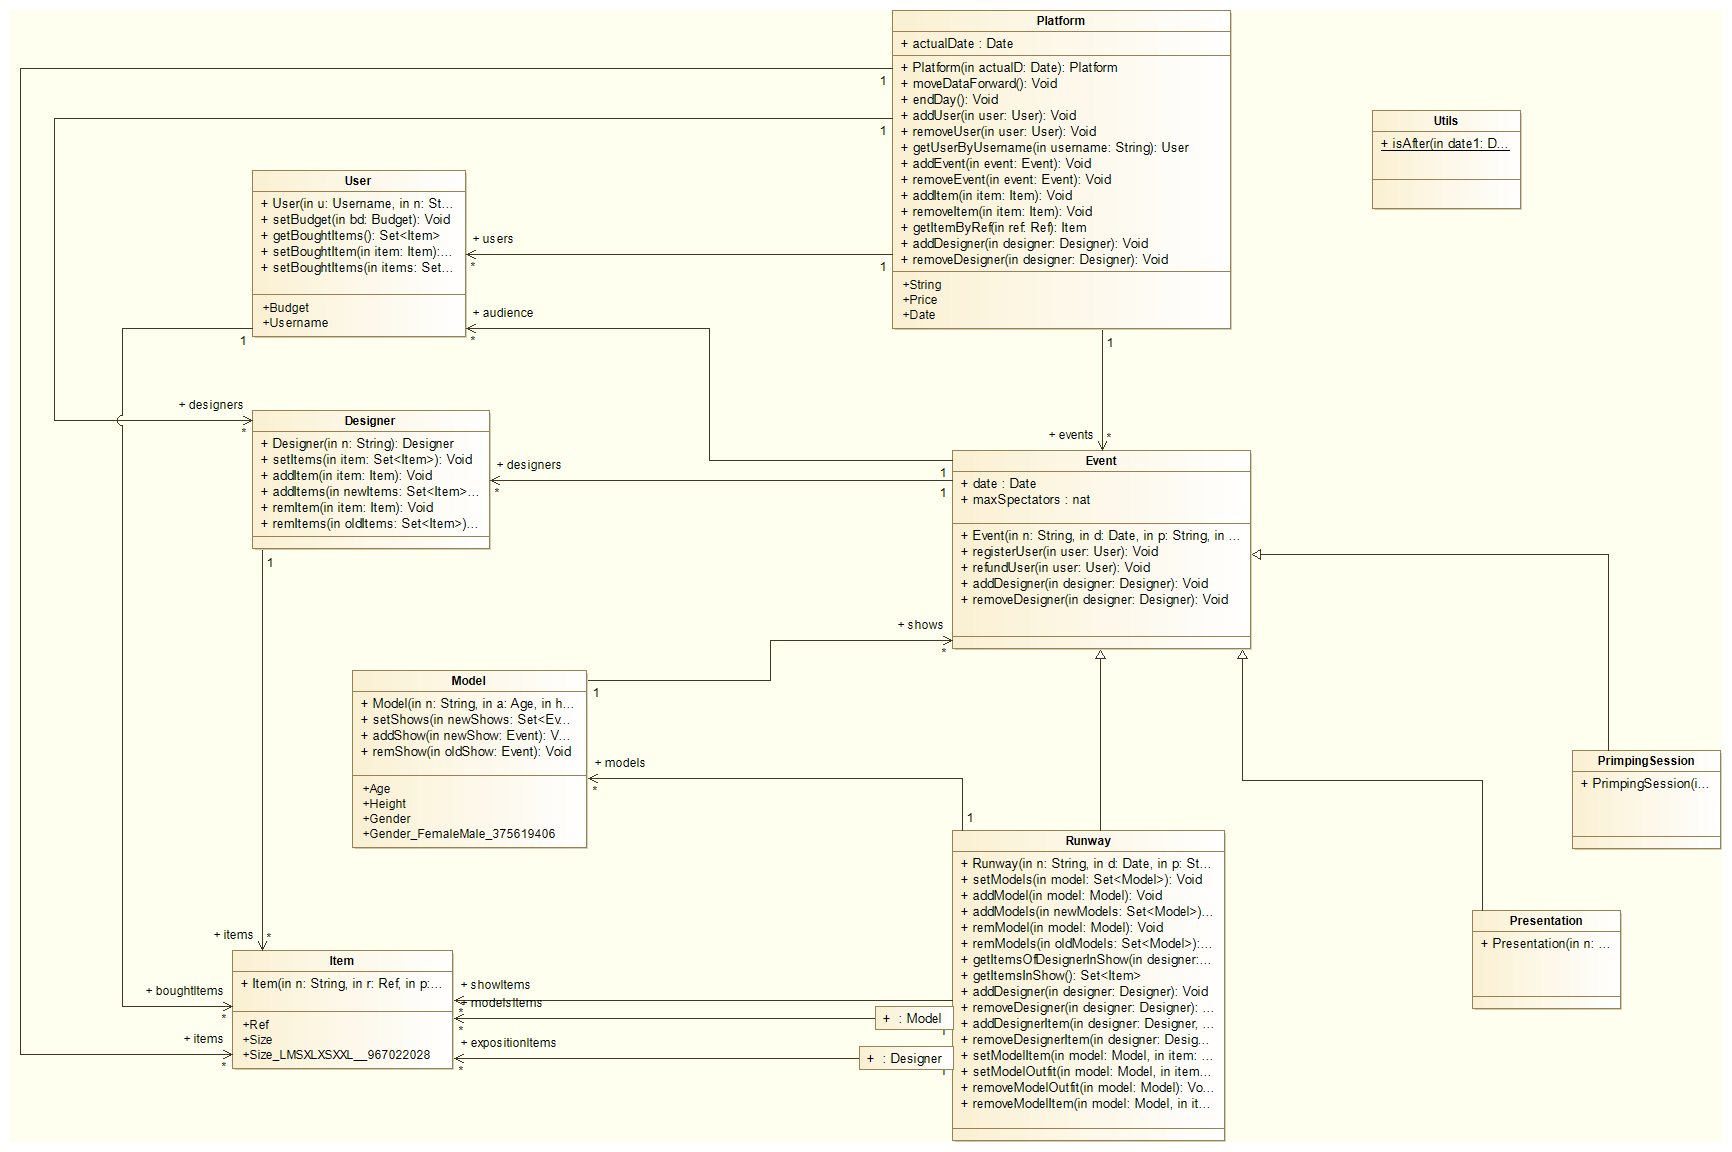
\includegraphics[width=160mm,height=150mm]{./images/class_diagram.png}
\caption{Diagrama de classes}
\label{fig:method}
\end{figure}
		
\section{Modelo Formal VDM++}
\subsection{Classe Platform}

\begin{vdmpp}[breaklines=true]
/**
* Esta classe representa a Plataforma de controlo de users, eventos, itens e designers 
*/
class Platform
types
  public String = seq of char
   inv s == s <> "";
  public Price = real 
   inv p == p > 0;
  public Date:: year : nat1
          month: nat1
         day  : nat1 
   inv d == d.month <= 12 and d.day <=30;
   
instance variables
 /**
 * data atual
 */
 public actualDate : Date;
 /**
 * users existentes numa plataforma
 */
 public users: set of User;
 inv not exists u1, u2 in set users & u1 <> u2 and u1.username = u2.username;
 /**
 * eventos existentes numa plataforma
 */
 public events: set of Event;
 inv not exists e1, e2 in set events & e1 <> e2 and e1.name = e2.name;
 inv not exists event in set events & Utils`isAfter(actualDate,event.date) = true;
 /**
 * itens existentes numa plataforma
 */
 public items: set of Item; 
 inv not exists i1, i2 in set items & i1 <> i2 and i1.reference = i2.reference;
 /**
 * designers existentes numa plataforma
 */
 public designers: set of Designer
 
 
operations
 /**
 * Plataform construtor
 * 
 * @param actualD corresponde a data atual da criacao de uma plataforma
 */
(*@
\label{Platform:48}
@*)
 public Platform:Date ==> Platform 
  Platform(actualD) == 
  (
   actualDate := actualD;
   users := {};
   events := {};
   items := {};
   designers := {};
   return self;
  );
-----------------------Date-----------------------------
 /**
 * Ajuste da data para com os limites de um mes, para ter datas reais
 */
(*@
\label{moveDataForward:62}
@*)
 public moveDataForward: () ==> ()
  moveDataForward() ==
  (
   if (actualDate.day + 1) > 30 then
   (
    actualDate.day := 1;
    if (actualDate.month+1) > 12 then
    (
     actualDate.month := 1;
     actualDate.year := actualDate.year + 1;
    )
    else
    (
     actualDate.month := actualDate.month + 1;
    );
   )
   else
   (
    actualDate.day := actualDate.day + 1;
   );
  );

 /**
 * Remocao de todos os eventos cujo dia da realizacao seja o atual
 */
(*@
\label{endDay:87}
@*)
 public endDay: () ==> ()
  endDay()==
  (
   moveDataForward();
   for all event in set events do 
   (
    if Utils`isAfter(actualDate,event.date) = true then
    (
     removeEvent(event);
    );
   );
  )
  pre not exists event in set events & Utils`isAfter(actualDate,event.date) = true
  post not exists event in set events & Utils`isAfter(actualDate,event.date) = true;



-----------------------Users----------------------------
 /*
 * Insercao de um user numa plataforma
 * 
 * @param user corresponde ao user a ser inserido nos users de uma plataforma
 */
(*@
\label{addUser:110}
@*)
 public addUser: User ==> ()
  addUser(user)==
  (
   users := users union {user};
  )
  pre user not in set users
  post user in set users and
  (not exists u1, u2 in set users & u1 <> u2 and u1.username = u2.username);
  
 /**
 * Remocao de um user dos users de uma plataforma
 * 
 * @param user corresponde ao user a ser removido dos users de uma plataforma
 */
(*@
\label{removeUser:124}
@*)
 public removeUser: User ==> ()
  removeUser(user)==
  (
   users := users \ {user};
  )
  pre user  in set users
  post user not in set users;


(*@
\label{getUserByUsername:133}
@*)
 public getUserByUsername: Platform`String ==> User
  getUserByUsername(username) ==
  (
   dcl user: User;
   for all u in set users do (
    if(u.username = username) then
     user := u;
   );
   return user;
  )
  post RESULT in set users;
-----------------------Events---------------------------
 /*
 * Insercao de um evento numa plataforma
 * 
 * @param event corresponde ao evento a ser inserido nos eventos de uma plataforma
 */
(*@
\label{addEvent:150}
@*)
 public addEvent: Event ==> ()
  addEvent(event)==
  (
   events := events union {event};
  )
  pre event not in set events
  post event in set events;
 
 /**
 * Remocao de um evento dos eventos de uma plataforma
 * 
 * @param event corresponde ao evento a ser removido dos eventos de uma plataforma
 */ 
(*@
\label{removeEvent:163}
@*)
 public removeEvent: Event ==> ()
  removeEvent(event)==
  (
   events := events \ {event};
  )
  pre event  in set events
  post event not in set events;
  
------------------------Items----------------------------
 /*
 * Insercao de um item numa plataforma
 * 
 * @param item corresponde ao item a ser inserido nos itens de uma plataforma
 */
(*@
\label{addItem:177}
@*)
 public addItem: Item ==> ()
  addItem(item)==
  (
   items := items union {item};
  )
  pre item not in set items
  post item in set items and
  (not exists i1, i2 in set items & i1 <> i2 and i1.reference = i2.reference);
  
 /**
 * Remocao de um item dos itens de uma plataforma
 * 
 * @param item corresponde ao item a ser removido dos itens de uma plataforma
 */ 
(*@
\label{removeItem:191}
@*)
 public removeItem: Item ==> ()
  removeItem(item)==
  (
   items := items \ {item};
  )
  pre item  in set items
  post item not in set items;
  
(*@
\label{getItemByRef:199}
@*)
 public getItemByRef: Item`Ref ==> Item
  getItemByRef(ref)== 
  (
   dcl item: Item ;
   for all it in set items do (
    if(it.reference = ref) then
     item := it;
   );
   return item;
  )
  post RESULT in set items;
----------------------Designers---------------------------
 /*
 * Insercao de um designer numa plataforma
 * 
 * @param designer corresponde ao designer a ser inserido nos designers de uma plataforma
 */
(*@
\label{addDesigner:216}
@*)
 public addDesigner: Designer ==> ()
  addDesigner(designer)==
  (
   designers := designers union {designer};
  )
  pre designer not in set designers
  post designer in set designers;
  
 /**
 * Remocao de um designer dos designers de uma plataforma
 * 
 * @param designer corresponde ao designer a ser removido dos designers de uma plataforma
 */ 
(*@
\label{removeDesigner:229}
@*)
 public removeDesigner: Designer ==> ()
  removeDesigner(designer)==
  (
   designers := designers \ {designer};
  )
  pre designer  in set designers
  post designer not in set designers;
 
----------------------------------------------------------------------
end Platform
\end{vdmpp}
\bigskip
\begin{longtable}{|l|r|r|r|}
\hline
Function or operation & Line & Coverage & Calls \\
\hline
\hline
\hyperref[Platform:48]{Platform} & 48&100.0\% & 9 \\
\hline
\hyperref[addDesigner:216]{addDesigner} & 216&100.0\% & 6 \\
\hline
\hyperref[addEvent:150]{addEvent} & 150&100.0\% & 18 \\
\hline
\hyperref[addItem:177]{addItem} & 177&100.0\% & 12 \\
\hline
\hyperref[addUser:110]{addUser} & 110&100.0\% & 57 \\
\hline
\hyperref[endDay:87]{endDay} & 87&100.0\% & 9 \\
\hline
\hyperref[getItemByRef:199]{getItemByRef} & 199&100.0\% & 3 \\
\hline
\hyperref[getUserByUsername:133]{getUserByUsername} & 133&100.0\% & 3 \\
\hline
\hyperref[moveDataForward:62]{moveDataForward} & 62&100.0\% & 3 \\
\hline
\hyperref[removeDesigner:229]{removeDesigner} & 229&100.0\% & 3 \\
\hline
\hyperref[removeEvent:163]{removeEvent} & 163&100.0\% & 15 \\
\hline
\hyperref[removeItem:191]{removeItem} & 191&100.0\% & 12 \\
\hline
\hyperref[removeUser:124]{removeUser} & 124&100.0\% & 12 \\
\hline
\hline
Platform.vdmpp & & 100.0\% & 162 \\
\hline
\end{longtable}


\subsection{Classe User}

\begin{vdmpp}[breaklines=true]
/**
* Esta classe representa o User e toda a informacao relacionada com ele, tal como atualizar o
* seu saldo e ver os itens comprados
*/
class User
types
 public Budget = real
  inv r == r >= 0.0;
 public Username = Platform`String;
 
values
-- TODO Define values here
instance variables
 /**
 * username sera unico, sendo a variavel de identificacao de um user
 */
 public username: Username;
 /**
 * nome de um user
 */
 public name: Platform`String;
 /**
 * saldo que permite a um user comprar itens ou inscrever-se em shows
 */
 public budget: Budget;
 /**
 * conjunto de itens comprados por um user
 */
 public boughtItems: set of Item;
operations
 /**
 * User construtor
 * 
 * @param u corresponde ao username de um user
 * @param n corresponde ao nome de um user
 */
(*@
\label{User:37}
@*)
 public User: Username * Platform`String ==> User 
 User(u,n) == 
 (
  username := u;
  name := n;
  budget := 0.0;
  boughtItems:= {};
  return self;
 );
 
 /**
 * Atualizacao do saldo de um user
 * 
 * @param bd corresponde ao saldo a inserir
 */
(*@
\label{setBudget:52}
@*)
 public setBudget: (Budget) ==> ()
  setBudget(bd) == budget := bd;
 /**
 * Deposito no saldo de um user
 * 
 * @param monet corresponde ao dinheiro a depositar
 */
(*@
\label{depositMoney:59}
@*)
 public depositMoney: Budget ==> ()
  depositMoney(money) ==
  (
   setBudget(budget + money);
  )
  pre money > 0.0
  post budget > 0.0;
 /**
 * Obtencao do conjunto de itens comprados por um user
 * 
 * @return set of Item
 */
(*@
\label{getBoughtItems:71}
@*)
 public getBoughtItems: () ==> set of Item
  getBoughtItems() == return boughtItems;
 
 /**
 * Atualizacao do conjunto de itens comprados por um user
 * 
 * @param item corresponde ao item a inserir no conjunto de itens de um user
 */
(*@
\label{setBoughtItem:79}
@*)
 public setBoughtItem: (Item) ==> ()
  setBoughtItem(item) == boughtItems := boughtItems union {item}
 post item in set boughtItems;
 
 /**
 * Atualizacao do conjunto de itens comprados por um user
 * 
 * @param items corresponde aos itens a inserir no conjunto de itens de um user
 */
(*@
\label{setBoughtItems:88}
@*)
 public setBoughtItems: (set of Item) ==> ()
  setBoughtItems(items) == boughtItems := boughtItems union items
 post items subset boughtItems ;
 
 /**
 * Compra um item ao utilizador
 *
 * @param item corresponde ao item a comprar
 */
(*@
\label{buyItem:97}
@*)
 public buyItem: (Item) ==> ()
  buyItem(item) == 
  (
   setBoughtItem(item);
   budget := budget - item.price;
  )
 pre budget >= item.price
 post budget >= 0;
 
functions
 
traces
-- TODO Define Combinatorial Test Traces here
end User
\end{vdmpp}
\bigskip
\begin{longtable}{|l|r|r|r|}
\hline
Function or operation & Line & Coverage & Calls \\
\hline
\hline
\hyperref[User:37]{User} & 37&100.0\% & 17 \\
\hline
\hyperref[buyItem:97]{buyItem} & 97&100.0\% & 1 \\
\hline
\hyperref[depositMoney:59]{depositMoney} & 59&100.0\% & 4 \\
\hline
\hyperref[getBoughtItems:71]{getBoughtItems} & 71&100.0\% & 12 \\
\hline
\hyperref[setBoughtItem:79]{setBoughtItem} & 79&100.0\% & 4 \\
\hline
\hyperref[setBoughtItems:88]{setBoughtItems} & 88&100.0\% & 3 \\
\hline
\hyperref[setBudget:52]{setBudget} & 52&100.0\% & 19 \\
\hline
\hline
User.vdmpp & & 100.0\% & 60 \\
\hline
\end{longtable}


\subsection{Classe Event}

\begin{vdmpp}[breaklines=true]
/**
* Esta classe representa um Evento e toda a informacao com ele relacionada, tal como
* os designers que estarao presentes ate aos users inscritos
*/  
class Event
values

instance variables
 /**
 * nome do evento
 */
 public name: Platform`String;
 /**
 * local onde se realizara o evento
 */
 public place: Platform`String;
 /**
 * data da realizacao do evento
 */
 public date: Platform`Date;
 /**
 * tema que descrevera o evento
 */
 public theme: Platform`String;
 /**
 * preco de entrada para o evento
 */
 public price: Platform`Price; 
 /**
 * designers que estarao a mostrar os seus itens no evento
 */
 public designers: set of Designer := {};
 /**
 * numero maximo de users inscritos para o evento
 */
 public maxSpectators: nat ;
 /**
 * users inscritos ate ao momento para o evento
 */
 public audience: set of User := {};

 inv ((card audience) >= 0) and ((card audience) <= maxSpectators);
 
operations
 /**
 * Event construtor
 * 
 * @param n corresponde ao nome de um evento
 * @param d corresponde a data de um evento
 * @param p corresponde ao local de um evento
 * @param t corresponde ao tema de um evento
 * @param pr corresponde ao preco de entrada de um evento
 * @param maxS corresponde ao numero maximo de users inscritos de um evento
 */
(*@
\label{Event:55}
@*)
 public Event: Platform`String * Platform`Date * Platform`String *  Platform`String * Platform`Price * nat ==> Event 
 Event(n,d, p, t, pr,  maxS) == 
 (
  name := n;
  date := d;
  place := p;
  theme := t;
  price := pr;
  maxSpectators := maxS;
  return self;
 );
----------------------------------------------------------------
 /**
 * Inscricao de um user no evento
 * 
 * @param user corresponde ao user a ser inscrito num evento
 */
(*@
\label{registerUser:72}
@*)
 public registerUser: User ==> ()
 registerUser(user) ==
 (
  audience := audience union {user};
  user.setBudget(user.budget - price);
 )
 pre (user.budget >= price) and
   (user not in set audience)
 post (user.budget >=0) and
    (card audience <= maxSpectators) and
    (user in set audience);
 
 /**
 * Remocao e reembolso de um user
 * 
 * @param user corresponde ao user a ser removido e reembolsado por um evento
 */
(*@
\label{refundUser:89}
@*)
 public refundUser: User ==> ()
 refundUser(user)==
 (
  audience := audience \ {user};
  user.setBudget(user.budget + price);
 )
 pre (user in set audience) and
   (user.budget >=0)
 
 post (user not in set audience) and
    (user.budget>0);

--------------------------------------------------------------
 /**
 * Adicao de um designer a um evento
 * 
 * @param designer corresponde ao designer a ser adicionado aos designer de um evento
 */
(*@
\label{addDesigner:107}
@*)
 public addDesigner: Designer ==> ()
 addDesigner(designer)==
 (
  designers:= designers union {designer};
 )
 pre designer not in set designers
 post designer in set designers;
 
 /**
 * Remocao de um designer
 * 
 * @param designer corresponde ao designer a ser removido dos designer de um evento
 */
(*@
\label{removeDesigner:120}
@*)
 public removeDesigner: Designer ==> ()
 removeDesigner(designer)==
 (
  designers:= designers \ {designer};
 )
 pre designer in set designers
 post designer not in set designers;
 
---------------------------------------------------------------
functions
-- TODO Define functiones here
traces
-- TODO Define Combinatorial Test Traces here
end Event
\end{vdmpp}
\bigskip
\begin{longtable}{|l|r|r|r|}
\hline
Function or operation & Line & Coverage & Calls \\
\hline
\hline
\hyperref[Event:55]{Event} & 55&100.0\% & 3 \\
\hline
\hyperref[addDesigner:107]{addDesigner} & 107&100.0\% & 6 \\
\hline
\hyperref[refundUser:89]{refundUser} & 89&100.0\% & 6 \\
\hline
\hyperref[registerUser:72]{registerUser} & 72&100.0\% & 9 \\
\hline
\hyperref[removeDesigner:120]{removeDesigner} & 120&100.0\% & 6 \\
\hline
\hline
Event.vdmpp & & 100.0\% & 30 \\
\hline
\end{longtable}


\subsection{Classe PrimpingSession}

\begin{vdmpp}[breaklines=true]
/**
* Esta classe representa a primping session
*/
class PrimpingSession is subclass of Event
types
-- TODO Define types here
values
-- TODO Define values here
instance variables
 
operations
 /**
 * PrimpingSession construtor
 */
(*@
\label{PrimpingSession:15}
@*)
 public PrimpingSession: Platform`String * Platform`Date * Platform`String *  Platform`String * Platform`Price * nat ==> PrimpingSession 
  PrimpingSession(n,d, p, t, pr,  maxS) == 
  (
   name := n;
   date := d;
   place := p;
   theme := t;
   price := pr;
   maxSpectators := maxS;
   return self;
  );
 
 
  
functions
end PrimpingSession
\end{vdmpp}
\bigskip
\begin{longtable}{|l|r|r|r|}
\hline
Function or operation & Line & Coverage & Calls \\
\hline
\hline
\hyperref[PrimpingSession:15]{PrimpingSession} & 15&100.0\% & 6 \\
\hline
\hline
PrimpingSession.vdmpp & & 100.0\% & 6 \\
\hline
\end{longtable}


\subsection{Classe Presentation}

\begin{vdmpp}[breaklines=true]
/**
* Esta classe representa uma Apresentacao
*/
class Presentation is subclass of Event
types
-- TODO Define types here
values
-- TODO Define values here
instance variables
 
operations
 /**
 * Presentation construtor
 */
(*@
\label{Presentation:15}
@*)
 public Presentation: Platform`String * Platform`Date * Platform`String *  Platform`String * Platform`Price * nat ==> Presentation 
  Presentation(n,d, p, t, pr,  maxS) == 
  (
   name := n;
   date := d;
   place := p;
   theme := t;
   price := pr;
   maxSpectators := maxS;
   return self;
  );
  
functions

end Presentation
\end{vdmpp}
\bigskip
\begin{longtable}{|l|r|r|r|}
\hline
Function or operation & Line & Coverage & Calls \\
\hline
\hline
\hyperref[Presentation:15]{Presentation} & 15&100.0\% & 6 \\
\hline
\hline
Presentation.vdmpp & & 100.0\% & 6 \\
\hline
\end{longtable}


\subsection{Classe Runway}

\begin{vdmpp}[breaklines=true]
/**
* Esta classe representa uma subclasse de um Evento, para ver  decorrer do evento 
*/
class Runway is subclass of Event
types

-- TODO Define types here
instance variables
 /**
 * itens de cada designer em exposicao
 */
 public expositionItems: map Designer to (set of Item) := {|->};
 /**
 * modelos disponiveis para usar desfilar com o itens dos designers
 */
  public models: set of Model := {};
  /**
 * itens a serem utilizados por cada modelo
 */
  public modelsItems: map Model to (set of Item) := {|->};
  /**
 * itens disponiveis no show
 */
  public showItems: set of Item := {};
operations
 /**
 * Runway construtor
 * 
 * @param n corresponde ao nome do evento
 * @param d corresponde a  data do evento
 * @param p corresponde ao local do evento
 * @param t corresponde ao tema do evento
 * @param pr corresponde ao preco de entrada do evento
 * @param maxS corresponde ao numero maximo de users inscritos no evento
 */
(*@
\label{Runway:36}
@*)
 public Runway: Platform`String * Platform`Date * Platform`String *  Platform`String * Platform`Price * nat ==>Runway
 Runway(n,d, p, t, pr, maxS)==
 (
  name := n;
  date := d;
  price := pr;
  theme := t;
  place := p;
  maxSpectators := maxS;
  return self;
 );
 
 /**
 * Insercaoo de modelos no conjunto de modelos do evento
 * 
 * @param model corresponde aos(as) modelos a serem inseridas num evento
 */
(*@
\label{setModels:53}
@*)
 public setModels: set of Model ==> ()
   setModels(model) == 
    models := model;
 
 /**
 * Insercao de um(a) modelo no conjunto de modelos do evento
 * 
 * @param model corresponde ao(a) modelo a ser inserida num evento
 */
(*@
\label{addModel:62}
@*)
 public addModel: Model ==> ()
  addModel(model) == (
     models := models union {model};
     modelsItems := modelsItems munion {model|-> {}};
  )
 pre model not in set models
 post model in set models;
 
 /**
 * Insercao de modelos no conjunto de modelos do evento
 * 
 * @param newModels corresponde aos(as) modelos a serem inseridas num evento
 */
(*@
\label{addModels:75}
@*)
 public addModels: set of Model ==> ()
  addModels(newModels) == (
    for all m in set newModels do (
      models := models union {m};
      modelsItems := modelsItems munion {m|-> {}};
   )
   )
 pre not newModels subset models
 post newModels subset models;
  
 /**
 * Remocao de um(a) modelo do evento
 * 
 * @param model corresponde ao(a) modelo a ser removida de um evento
 */
(*@
\label{remModel:90}
@*)
 public remModel: Model ==> ()
  remModel(model) == (
     models := models \ {model}
   )
 pre models <> {} and model in set models
 post model not in set models;
 
 /**
 * Remocao de um conjunto de modelos do evento
 * 
 * @param oldModels corresponde aos(as) modelos a serem removidas
 */
(*@
\label{remModels:102}
@*)
 public remModels: set of Model ==> ()
  remModels(oldModels) == (
    for all model in set oldModels do (
      models := models \ {model};
    )
  )
 pre models <> {} and oldModels subset models
 post not oldModels subset models;
 
 /**
 * Dado um designer obtem-se o conjunto de itens que ele dispoe
 * 
 * @param designer corresponde ao designer de quem se quer obter os itens
 * @return conjunto de itens
 */
(*@
\label{getItemsOfDesignerInShow:117}
@*)
 public getItemsOfDesignerInShow: Designer ==> set of Item
 getItemsOfDesignerInShow(designer) ==
 (
  return expositionItems(designer);
 )
 pre designer in set dom expositionItems;
 
 /**
 * Obter os itens disponiveis no show
 * 
 * @return conjunto de itens
 */
(*@
\label{getItemsInShow:129}
@*)
 public getItemsInShow:() ==> set of Item
 getItemsInShow() ==
 (
  dcl items: set of Item := {};
  for all item in set rng expositionItems do (
   items := items union item;
  );
  showItems := items;
  return items;
 );

-------------------------------------------------------------
 /**
 * Adicao de um designer no conjunto de designers, bem como atualizacao 
 * dos itens do show e dos itens em exposicao
 * 
 * @param designer corresponde ao designer a adicionar ao evento
 */
(*@
\label{addDesigner:147}
@*)
 public addDesigner: Designer ==> ()
 addDesigner(designer)==
 (
  designers := designers union {designer};
  showItems := showItems union designer.items;
  expositionItems := expositionItems munion {designer|-> designer.items};
  
 )
 pre (designer not in set designers) and
   (designer not in set dom expositionItems)
 
 post (designer  in set designers) and
    (designer  in set dom expositionItems); 
 
 /**
 * Remocao de um designer do conjunto de designers, bem como atualizacao
 * dos itens do shwo e dos itens em exposicao
 * 
 * @param designer corresponde ao designer a remover do evento
 */
(*@
\label{removeDesigner:167}
@*)
 public removeDesigner: Designer ==> ()
 removeDesigner(designer)==
 (
  designers:= designers \ {designer};
  showItems := showItems \ designer.items;
  expositionItems:= {designer} <-: expositionItems;
 )
 pre (designer  in set designers) and
   (designer  in set dom expositionItems) 
 post (designer not in set designers) and
    (designer not in set dom expositionItems);
-------------------------------------------------------------    
 /**
 * Adicao de um item associado a um designer aos itens do show e aos itens em exposicao
 * 
 * @param designer corresponde ao designer de quem o item a ser inserido pertence
 * @param item corresponde ao item a ser inserido no evento
 */
(*@
\label{addDesignerItem:185}
@*)
 public addDesignerItem: Designer * Item ==> ()
 addDesignerItem(designer,item)==
 (
   showItems := showItems union {item};
   expositionItems(designer):= expositionItems(designer) union {item};
 )
 pre (designer in set designers) and
   (designer in set (dom expositionItems)) and
   (item not in set expositionItems(designer))
 post item in set expositionItems(designer);
 
 /**
 * Remocao de um item associado a um designer dos itens do show e dos itens em exposicao
 * 
 * @param designer corresponde ao designer de quem o item a ser removido pertence
 * @param item corresponde ao item a ser removido do evento
 */
(*@
\label{removeDesignerItem:202}
@*)
 public removeDesignerItem: Designer * Item ==> ()
 removeDesignerItem(designer,item)==
 (
  showItems := showItems \ {item};
  expositionItems(designer):= expositionItems(designer) \ {item};
 )
 pre (designer in set designers) and
   (designer in set dom expositionItems) and
   (item in set expositionItems(designer))
 post item not in set expositionItems(designer);
 
 --public addItemByRef: Item`Ref ==> ()
 --addItemByRef(ref) ==
 --(
 -- for all designer in set designers do
 -- (
 --  for all item in set designer.items do
 --  (
 --   if item.reference = ref 
 --   then addDesignerItem(designer,item);
 --  )
 -- )
 --);
------------------------------------------------------------
------------------------------------------------------------- 
 /**
 * Adicao de um item aos itens que um(a) modelo utilizara no evento
 * 
 * @param model corresponde ao(a) modelo a quem o item vai ser associado
 * @param item corresponde ao item a ser adicionado
 */   
(*@
\label{setModelItem:233}
@*)
 public setModelItem: Model * Item ==> ()
 setModelItem(model,item)==
 (
   modelsItems(model):= modelsItems(model) union {item};
 )
 pre (model in set models) and
   (model in set (dom modelsItems)) and
   (item not in set modelsItems(model)) and
   item in set showItems
 post item in set modelsItems(model);
 
 /**
 * Adicao de um conjunto de itens(Outfit) aos itens a serem utilizados por um(a) modelo
 * 
 * @param model corresponde ao(a) modelo a quem os itens vao ser adicionados
 * @param items corresponde aos itens a serem adicionados
 */
(*@
\label{setModelOutfit:250}
@*)
 public setModelOutfit: Model * set of Item ==> ()
 setModelOutfit(model,items)==
 (
   modelsItems(model):= modelsItems(model) union items;
 )
 pre (model in set models) and
   (model in set (dom modelsItems)) and
   (not (items  subset modelsItems(model)))
 post items subset modelsItems(model);
 
 /**
 * Remocao de um conjunto de itens(Outfi) dos itens que um(a) modelo tinha associado para o evento
 * 
 * @param model corresponde ao(a) modelo a quem o item vai ser removido
 * @param item corresponde ao itens a serem removidos
 */
(*@
\label{removeModelOutfit:266}
@*)
 public removeModelOutfit: Model ==> ()
 removeModelOutfit(model)==
 (
  modelsItems:= {model} <-: modelsItems;
  modelsItems := modelsItems munion {model|-> {}};
 )
 pre (model in set models) and
   (model in set dom modelsItems);
 
 /**
 * Remocao de um item dos itens que um(a) modelo tinha associado para o evento
 * 
 * @param model corresponde ao(a) modelo a quem o item vai ser removido
 * @param item corresponde ao item a ser removido
 */ 
(*@
\label{removeModelItem:281}
@*)
 public removeModelItem: Model * Item ==> ()
 removeModelItem(model,item)==
 (
  modelsItems(model):= modelsItems(model) \ {item};
 )
 pre (model in set models) and
   (model in set dom modelsItems) and
   (item in set modelsItems(model))
 post item not in set modelsItems(model);
end Runway
\end{vdmpp}
\bigskip
\begin{longtable}{|l|r|r|r|}
\hline
Function or operation & Line & Coverage & Calls \\
\hline
\hline
\hyperref[Runway:36]{Runway} & 36&100.0\% & 78 \\
\hline
\hyperref[addDesigner:147]{addDesigner} & 147&100.0\% & 57 \\
\hline
\hyperref[addDesignerItem:185]{addDesignerItem} & 185&100.0\% & 3 \\
\hline
\hyperref[addModel:62]{addModel} & 62&100.0\% & 3 \\
\hline
\hyperref[addModels:75]{addModels} & 75&100.0\% & 45 \\
\hline
\hyperref[getItemsInShow:129]{getItemsInShow} & 129&100.0\% & 6 \\
\hline
\hyperref[getItemsOfDesignerInShow:117]{getItemsOfDesignerInShow} & 117&100.0\% & 18 \\
\hline
\hyperref[remModel:90]{remModel} & 90&100.0\% & 3 \\
\hline
\hyperref[remModels:102]{remModels} & 102&100.0\% & 6 \\
\hline
\hyperref[removeDesigner:167]{removeDesigner} & 167&100.0\% & 3 \\
\hline
\hyperref[removeDesignerItem:202]{removeDesignerItem} & 202&100.0\% & 3 \\
\hline
\hyperref[removeModelItem:281]{removeModelItem} & 281&100.0\% & 3 \\
\hline
\hyperref[removeModelOutfit:266]{removeModelOutfit} & 266&100.0\% & 6 \\
\hline
\hyperref[setModelItem:233]{setModelItem} & 233&100.0\% & 6 \\
\hline
\hyperref[setModelOutfit:250]{setModelOutfit} & 250&100.0\% & 18 \\
\hline
\hyperref[setModels:53]{setModels} & 53&100.0\% & 12 \\
\hline
\hline
Runway.vdmpp & & 100.0\% & 270 \\
\hline
\end{longtable}


\subsection{Classe Model}

\begin{vdmpp}[breaklines=true]
/**
* Esta classe representa um(a) Modelo bem como os shows nos quais esta associada para participar
*/
class Model
types
 public Age = int
  inv i ==  i <= 65 and  i >= 18;
 public Height = real 
  inv r == r <= 2.10 and r >= 1.60;
 public Gender = <Female>|<Male>;
values
-- TODO Define values here
instance variables
 /**
 * nome de um(a) modelo
 */ 
 public name:  Platform`String;
 /**
 * idade de um(a) modelo
 */
 public age: Age;
 /**
 * peso de um(a) modelo
 */
 public height: Height;
 /**
 * nacionalidade de um(a) modelo
 */ 
 public nationality: Platform`String;
 /**
 * shows nos quais um(a) modelo vai participar
 */
 public shows: set of Event;
 /**
 * genero de um(a) modelo
 */
 public gender: Gender;
 
 inv card shows >= 0;
 
operations
 /**
 * Model construtor
 * 
 * @param n corresponde ao nome de um(a) modelo
 * @param a corresponde a  idade de um(a) modelo
 * @param h corresponde ao peso de um(a) modelo
 * @param na corresponde a  nacionalidade de um(a) modelo
 * @param g corresponde ao genero de um(a) modelo
 */
(*@
\label{Model:51}
@*)
 public Model: Platform`String * Age * Height * Platform`String * Gender ==> Model 
 Model(n, a, h, na, g) == 
 (
  name := n;
  age := a;
  height := h;
  nationality := na;
  shows := {};
  gender := g;
  return self;
 );
 
 /**
 * Insercao de um(a) modelo em shows, que ficam visiveis nos shows de um(a) modelo
 * 
 * @param newShows corresponde aos shows a serem adicionados aos shows de um(a) modelo
 */
(*@
\label{setShows:68}
@*)
 public setShows: set of Event ==> ()
  setShows(newShows) == (
   shows := newShows;
  )
 pre shows = {}
 post shows = newShows;
 
 /**
 * Insercao de um(a) modelo num show que ficara visivel nos shows de um(a) modelo
 * 
 * @param newShow corresponde ao show a ser adicionado aos shows de um(a) modelo
 */
(*@
\label{addShow:80}
@*)
 public addShow: Event ==> ()
  addShow(newShow) == (
     shows := shows union {newShow}
 )
 pre newShow not in set shows 
  and forall s in set shows & (newShow.date.day <> s.date.day or
                 newShow.date.month <> s.date.month or
                  newShow.date.year <> s.date.year)
 post newShow in set shows;
 
 /**
 * Remocaoo de um(a) modelo de um show que deixara de estar visivel nos shows de um(a) modelo
 * 
 * @param oldShow corresponde ao show a ser removido dos shows de um(a) modelo
 */
(*@
\label{remShow:95}
@*)
 public remShow: Event ==> ()
  remShow(oldShow) == (
   shows := shows \ {oldShow}
  )
  pre oldShow in set shows
  and shows <> {}
  post oldShow not in set shows;
  
functions
-- TODO Define functiones here

end Model
\end{vdmpp}
\bigskip
\begin{longtable}{|l|r|r|r|}
\hline
Function or operation & Line & Coverage & Calls \\
\hline
\hline
\hyperref[Model:51]{Model} & 51&100.0\% & 60 \\
\hline
\hyperref[addShow:80]{addShow} & 80&100.0\% & 9 \\
\hline
\hyperref[remShow:95]{remShow} & 95&100.0\% & 3 \\
\hline
\hyperref[setShows:68]{setShows} & 68&100.0\% & 9 \\
\hline
\hline
Model.vdmpp & & 100.0\% & 81 \\
\hline
\end{longtable}


\subsection{Classe Designer}
\begin{vdmpp}[breaklines=true]
/**
* Esta classe representa um Designer bem como os itens que dispoe para os shows
*/
class Designer
types

instance variables
  /**
  * nome do designer
  */
  public name: Platform`String;
  /**
  * itens dos quais o designer dispoe
  */
  public items: set of Item;
values
 
operations
 /**
 * Designer construtor
 * 
 * @param n nome de um designer
 */
(*@
\label{Designer:24}
@*)
 public Designer: Platform`String ==> Designer 
  Designer(n) == (
   name := n;
   items := {};
   return self;
 );
 
 /**
 * Insercao de um conjunto de itens nos itens de um designer
 * 
 * @param item corresponde aos itens a serem inseridos
 */
(*@
\label{setItems:36}
@*)
 public setItems: set of Item ==> ()
   setItems(item) == 
    items := item;
    
 /**
 * Insercao de um item no conjunto de itens de um designer
 * 
 * @param item corresponde ao item a ser inserido
 */
(*@
\label{addItem:45}
@*)
 public addItem: Item ==> ()
  addItem(item) == (
     items := items union {item}
  )
 pre item not in set items
 post item in set items;
 
 /**
 * Insercao de um conjunto de itens nos itens de um designer
 * 
 * @param newItems corresponde aos itens a serem inseridos
 */
(*@
\label{addItems:57}
@*)
 public addItems: set of Item ==> ()
  addItems(newItems) == (
    for all i in set newItems do (
      items := items union {i};
    )
   )
 pre (not newItems subset items) and newItems <> items
 post newItems subset items;
   
  /**
 * Remocao de um item do conjunto de itens de um designer
 * 
 * @param item corresponde ao item a ser removido
 */
(*@
\label{remItem:71}
@*)
 public remItem: Item ==> ()
  remItem(item) ==
      items := items \ {item}
 pre items <> {} and item in set items
 post item not in set items;
  
 /**
 * Remocao de um conjunto de itens dos itens de um designer
 * 
 * @param oldItems corresponde aos itens a serem removidos
 */
(*@
\label{remItems:82}
@*)
 public remItems: set of Item ==> ()
  remItems(oldItems) ==
    for all i in set oldItems do (
      items := items \ {i}
    )
 pre items <> {} and (oldItems subset items)
 post not oldItems subset items;
  
functions

end Designer

\end{vdmpp}
\bigskip
\begin{longtable}{|l|r|r|r|}
\hline
Function or operation & Line & Coverage & Calls \\
\hline
\hline
\hyperref[Designer:24]{Designer} & 24&100.0\% & 117 \\
\hline
\hyperref[addItem:45]{addItem} & 45&100.0\% & 3 \\
\hline
\hyperref[addItems:57]{addItems} & 57&100.0\% & 57 \\
\hline
\hyperref[remItem:71]{remItem} & 71&100.0\% & 3 \\
\hline
\hyperref[remItems:82]{remItems} & 82&100.0\% & 3 \\
\hline
\hyperref[setItems:36]{setItems} & 36&100.0\% & 12 \\
\hline
\hline
Designer.vdmpp & & 100.0\% & 195 \\
\hline
\end{longtable}


\subsection{Class Item}

\begin{vdmpp}[breaklines=true]
/**
* Esta classe representa um Item contendo toda a informacao relacionada com um Item
*/
class Item
types
 public Ref =  seq of char 
 inv v == len v = 9;
 public Size = <XS>|<S>|<M>|<L>|<XL>|<XXL>;

instance variables
 /**
 * nome de um item
 */
 public name: Platform`String;
 /**
 * referencia associada a um item
 */
 public reference: Ref;
 /**
 * preco de um item
 */
 public price: Platform`Price;
 /**
 * tamanho de um item 
 */
 public size: Size;

operations
 /**
 * Item construtor
 * 
 * @param n corresponde ao nome de um item
 * @param r corresponde a referencia de um item
 * @param p corresponde ao preco de um item
 * @param s corresponde ao tamanho de um item
 */
(*@
\label{Item:37}
@*)
 public Item: Platform`String * Ref * Platform`Price * Size ==> Item 
  Item(n, r, p, s) == 
  (
   name := n;
   reference := r;
   price := p;
   size := s;
   return self;
  );
  
functions
 -- TODO Define functiones here
end Item
\end{vdmpp}
\bigskip
\begin{longtable}{|l|r|r|r|}
\hline
Function or operation & Line & Coverage & Calls \\
\hline
\hline
\hyperref[Item:37]{Item} & 37&100.0\% & 69 \\
\hline
\hline
Item.vdmpp & & 100.0\% & 69 \\
\hline
\end{longtable}


\subsection{Classe Utils}

\begin{vdmpp}[breaklines=true]
/**
* Esta classe representa as funcoes uilitarias e comuns a todas as classes
*/
class Utils
types
-- TODO Define types here
values
-- TODO Define values here
instance variables
-- TODO Define instance variables here
operations
 
functions
 /**
 * Verifica duas datas de modo a comparar se a primeira e posterior a segunda
 * 
 * @param data1 corresponde a primeira data
 * @param data2 corresponde a segunda data
 */
(*@
\label{isAfter:20}
@*)
 public isAfter: Platform`Date * Platform`Date -> bool
  isAfter(date1, date2) ==
  (
   if date1.year > date2.year then
    true
   elseif date1.year < date2.year then 
    false
   else 
   (
    if date1.month > date2.month then
     (*@\vdmnotcovered{true}@*)
    elseif date1.month < date2.month then
     true
    else 
    (
     if date1.day > date2.day then
      true
     else 
      false
    )
   )
  );
traces
-- TODO Define Combinatorial Test Traces here
end Utils
\end{vdmpp}
\bigskip
\begin{longtable}{|l|r|r|r|}
\hline
Function or operation & Line & Coverage & Calls \\
\hline
\hline
\hyperref[isAfter:20]{isAfter} & 20&97.0\% & 36 \\
\hline
\hline
Utils.vdmpp & & 97.0\% & 36 \\
\hline
\end{longtable}



\section{Modelo de Validação}
\subsection{Classe Test}
\begin{vdmpp}[breaklines=true]
class Test is subclass of MyTestCase
instance variables

 d1: Designer := (*@\vdmnotcovered{new}@*) (*@\vdmnotcovered{Designer}@*)((*@\vdmnotcovered{"Miguel Lira"}@*));
 d2: Designer := new Designer((*@\vdmnotcovered{"Miriam Gon�alves"}@*));
 d3: Designer := (*@\vdmnotcovered{new}@*) (*@\vdmnotcovered{Designer}@*)((*@\vdmnotcovered{"Paulo S�rgio"}@*));
 d4: Designer := (*@\vdmnotcovered{new}@*) (*@\vdmnotcovered{Designer}@*)((*@\vdmnotcovered{"Coco Chanel"}@*));
 d5: Designer := new (*@\vdmnotcovered{Designer}@*)((*@\vdmnotcovered{"Ralph Lauren"}@*));
 d6: Designer := new Designer((*@\vdmnotcovered{"Karl Lagerfeld"}@*));
 d7: Designer := (*@\vdmnotcovered{new}@*) (*@\vdmnotcovered{Designer}@*)((*@\vdmnotcovered{"Donatella Versace"}@*));
 
 
 u1: User := new User("zequinhaBombeiro",(*@\vdmnotcovered{"Jos� Esteves"}@*));
 u2: User := new (*@\vdmnotcovered{User}@*)((*@\vdmnotcovered{"digas"}@*),(*@\vdmnotcovered{"Diogo Coelho"}@*));
 u3: User := (*@\vdmnotcovered{new}@*) (*@\vdmnotcovered{User}@*)((*@\vdmnotcovered{"loirinha33"}@*),(*@\vdmnotcovered{"Anabela Costa"}@*));
 
 m1: Model:= (*@\vdmnotcovered{new}@*) (*@\vdmnotcovered{Model}@*)((*@\vdmnotcovered{"Adriana Lima"}@*), 36, (*@\vdmnotcovered{1.78}@*), (*@\vdmnotcovered{"Brasil"}@*), (*@\vdmnotcovered{<Female>}@*));
 m2: Model:= new Model("Sara Sampaio", 26, (*@\vdmnotcovered{1.72}@*), (*@\vdmnotcovered{"Portugal"}@*), (*@\vdmnotcovered{<Female>}@*));
 m3: Model:= (*@\vdmnotcovered{new}@*) (*@\vdmnotcovered{Model}@*)((*@\vdmnotcovered{"Karlie Kloss"}@*), (*@\vdmnotcovered{25}@*), (*@\vdmnotcovered{1.88}@*), (*@\vdmnotcovered{"U.S.A"}@*), (*@\vdmnotcovered{<Female>}@*));
 m4: Model:= new (*@\vdmnotcovered{Model}@*)((*@\vdmnotcovered{"Gigi Hadid"}@*), (*@\vdmnotcovered{22}@*), (*@\vdmnotcovered{1.79}@*), (*@\vdmnotcovered{"U.S.A"}@*), (*@\vdmnotcovered{<Female>}@*));
 m5: Model:= new Model("Candice Swanepoel", 29, 1.77, (*@\vdmnotcovered{"Africa do Sul"}@*), (*@\vdmnotcovered{<Female>}@*));
 m6: Model:= new Model((*@\vdmnotcovered{"Lily Aldridge"}@*), 32, (*@\vdmnotcovered{1.75}@*), (*@\vdmnotcovered{"U.S.A"}@*), (*@\vdmnotcovered{<Female>}@*));
 m7: Model:= (*@\vdmnotcovered{new}@*) (*@\vdmnotcovered{Model}@*)((*@\vdmnotcovered{"Ashley Graham"}@*), 30, (*@\vdmnotcovered{1.75}@*), (*@\vdmnotcovered{"U.S.A"}@*), (*@\vdmnotcovered{<Female>}@*));
 m8: Model:= new Model("Miles McMillan", 28, (*@\vdmnotcovered{1.88}@*), (*@\vdmnotcovered{"U.S.A"}@*), (*@\vdmnotcovered{<Male>}@*));
 
 it1: Item := new Item("Camisolinha de l�","1c34ff445",220.50,(*@\vdmnotcovered{<XL>}@*));
 it2: Item := new Item("Oculos de Sol Gucci",(*@\vdmnotcovered{"123ggg4hk"}@*),(*@\vdmnotcovered{220.50}@*),(*@\vdmnotcovered{<S>}@*));
 it3: Item := new (*@\vdmnotcovered{Item}@*)((*@\vdmnotcovered{"Calcinha Branca"}@*),(*@\vdmnotcovered{"1c34ff445"}@*),(*@\vdmnotcovered{220.50}@*),(*@\vdmnotcovered{<M>}@*));
 it4: Item := new Item("Camisola Sarja Preta Versace",(*@\vdmnotcovered{"3213fff23"}@*),(*@\vdmnotcovered{220.50}@*),(*@\vdmnotcovered{<L>}@*));
 it5: Item := new Item("Camisolinha de l�","1c34ff445",(*@\vdmnotcovered{220.50}@*),(*@\vdmnotcovered{<XS>}@*));
 it6: Item := new Item((*@\vdmnotcovered{"Camisolinha de l�"}@*),(*@\vdmnotcovered{"1c34ff445"}@*),220.50,(*@\vdmnotcovered{<XS>}@*));
 it7: Item := new (*@\vdmnotcovered{Item}@*)("Camisolinha de l�","1c34ff445",220.50,(*@\vdmnotcovered{<S>}@*));
 it8: Item := new Item("Camisolinha de l�",(*@\vdmnotcovered{"1c34ff445"}@*),220.50,(*@\vdmnotcovered{<M>}@*));
 
operations
(*@
\label{main:36}
@*)
public static main: () ==> ()
 main() == (
 IO`println("Inicializar testes...");
  new TestDesignerClass().testAll();
  new TestModelClass().testAll();
  new TestItemClass().testAll();
  new TestUserClass().testAll();
  new TestPrimpingSessionClass().testAll();
  new TestPresentationClass().testAll();
  new TestEventClass().testAll();
  new TestPlatformClass().testAll();
  new TestUtilsClass().testAll();  
  new TestRunwayClass().testAll();
  IO`println("Testes terminados com sucesso!");
 );

end Test
\end{vdmpp}
\bigskip
\begin{longtable}{|l|r|r|r|}
\hline
Function or operation & Line & Coverage & Calls \\
\hline
\hline
\hyperref[main:36]{main} & 36&100.0\% & 2 \\
\hline
\hline
test.vdmpp & & 9.8\% & 2 \\
\hline
\end{longtable}



\subsection{Classe MyTestCase}
\begin{vdmpp}[breaklines=true]
/*
 * Superclass for test classes, simpler but more practical than VDMUnit`TestCase.
 * For proper use, you have to do: New -> Add VDM Library -> IO.
 * JPF, FEUP, MFES, 2014/15.
 */
class MyTestCase
operations

  /**
   * Simulates assertion checking by reducing it to pre-condition checking.
   * If 'arg' does not hold, a pre-condition violation will be signaled.
   */
(*@
\label{assertTrue:13}
@*)
  protected assertTrue: bool ==> ()
  assertTrue(arg) ==
    (*@return@*)
  pre (*@arg@*);

  /**
   * Simulates assertion checking by reducing it to post-condition checking.
   * If values are not equal, prints a message in the console and generates
   * a post-conditions violation.
   */
(*@
\label{assertEqual:23}
@*)
  protected assertEqual: ? * ? ==> ()
  assertEqual(expected, actual) ==
    if expected <> actual then (*@(@*)
      (*@IO`print@*)((*@"Actual value ("@*));
      (*@IO`print@*)((*@actual@*));
      (*@IO`print@*)((*@") different from expected ("@*));
      IO`print((*@expected@*));
      IO`println((*@")\textbackslash n"@*))
    )
  post expected = actual

end MyTestCase
\end{vdmpp}




\subsection{Classe TestPlatformClass}
\begin{vdmpp}[breaklines=true]
class TestPlatformClass is subclass of MyTestCase
types
-- TODO Define types here
values
-- TODO Define values here
instance variables
 
 d1: Designer := new Designer("Oscar de La Renta");
 d2: Designer := new Designer("Donna Karen");
 d3: Designer := new Designer("Alexander McQueen");
 
 it1: Item := new Item("Camisolinha de l�","1c34ff445",220.50,<XL>);
 it2: Item := new Item("Oculos de Sol Gucci","123ggg4hk",220.50,<S>);
 it3: Item := new Item("Calcinha Branca","1c34ff445",220.50,<M>);
 
 u1: User := new User("mitchLira", "Miguel Lira");
 u2: User := new User("miriniri", "Miriam Goncalves");
 u3: User := new User("pauloB", "Paulo Babo");
 

 e1: Event := new PrimpingSession("Fique Bela e Amarela",mk_Platform`Date(2017,12,29),"Avenida dos Aliados","Amarelo/Dourado",
                  20,50);
 e2: Event := new Presentation("Como andar na moda?",
                 mk_Platform`Date(2018,1,5),
                 "Antigas Fabricas Tabopan",
                 "Moda",
                 5,
                 300);
 e3: Event := new Runway("Victoria's Secret Runway",
              mk_Platform`Date(2018,2,22),
              "Covelo de Ansi�es",
              "Langerie",
              300,
              50
              );
 e4: Event := new Runway("Gigi vs Tommy Runway",
              mk_Platform`Date(2018,12,30),
              "Amarante",
              "Funny",
              300,
              50
              );
 
 e5: Event := new Runway("Gucci for poor",
              mk_Platform`Date(2019,11,30),
              "Guimar�es",
              "Pobreza",
              300,
              50
              );                          
 p1: Platform := new Platform(mk_Platform`Date(2017,12,29));
 p2: Platform := new Platform(mk_Platform`Date(2018,12,30));
 p3: Platform := new Platform(mk_Platform`Date(2017,11,30));
operations
(*@
\label{testAddRemoveDesigner:55}
@*)
 public testAddRemoveDesigner: () ==> ()
 testAddRemoveDesigner()==
 (
    IO`println("\t (1) Adi��o e remo��o de um designer da plataforma");
  p1.addDesigner(d1);
  p1.addDesigner(d2);
  assertEqual({d1,d2},p1.designers);
  p1.removeDesigner(d2);
  assertEqual({d1},p1.designers);
 );
 
(*@
\label{testAddRemoveItem:66}
@*)
 public testAddRemoveItem: () ==> ()
 testAddRemoveItem()==
 (
  IO`println("\t (2) Adi��o e remo��o de um item da plataforma");
  p1.addItem(it1);
  p1.addItem(it2);
  assertEqual({it1,it2},p1.items);
  p1.removeItem(it2);
  p1.removeItem(it1);
  assertEqual({},p1.items);
 );
 
(*@
\label{testAddRemoveUser:78}
@*)
 public testAddRemoveUser: () ==> ()
 testAddRemoveUser()==
 (
  IO`println("\t (3) Adi��o e remo��o de um utilizador da plataforma");
  p1.addUser(u1);
  p1.addUser(u2);
  assertEqual({u1,u2},p1.users);
  p1.removeUser(u2);
  p1.removeUser(u1);
  assertEqual({},p1.users);
 );
 
(*@
\label{testAddRemoveEvent:90}
@*)
 public testAddRemoveEvent: () ==> ()
 testAddRemoveEvent()==
 (
  IO`println("\t (4) Adi��o e remo��o de um evento da plataforma");
  p1.addEvent(e1);
  p1.addEvent(e2);
  assertEqual({e1,e2},p1.events);
  p1.removeEvent(e2);
  p1.removeEvent(e1);
  assertEqual({},p1.events);
 );
 
 
(*@
\label{testEndDay:103}
@*)
 public testEndDay: () ==> ()
 testEndDay()==
 ( IO`println("\t (5) Finaliza��o de um dia de eventos");
  p1.addEvent(e1);
  p1.addEvent(e2);
  p1.endDay();
  assertEqual(30,p1.actualDate.day);
  assertEqual(12,p1.actualDate.month);
  assertEqual(2017,p1.actualDate.year);
  assertEqual({e2},p1.events);
  p2.addEvent(e4);
  p2.endDay();
  assertEqual(1,p2.actualDate.day);
  assertEqual(1,p2.actualDate.month);
  assertEqual(2019,p2.actualDate.year);
  p1.removeEvent(e2);
  p3.addEvent(e5);
  p3.endDay();
  assertEqual(1,p3.actualDate.day);
  assertEqual(12,p3.actualDate.month);
  assertEqual(2017,p3.actualDate.year);
 );
 
(*@
\label{testgetItemByRef:126}
@*)
 public testgetItemByRef: () ==> ()
 testgetItemByRef()==
 (
  IO`println("\t (6) Selecionar um item pela refer�ncia");
  p1.addItem(it1);
  p1.addItem(it2);
  assertEqual(p1.getItemByRef("123ggg4hk"), it2);
 );
 
(*@
\label{testgetUserByUsername:135}
@*)
 public testgetUserByUsername: () ==> ()
  testgetUserByUsername()==
  (
   IO`println("\t (6) Selecionar um utilizador pelo username");
   p1.addUser(u1);
   p1.addUser(u2);
   p1.addUser(u3);
   assertEqual(p1.getUserByUsername("pauloB"), u3);
  );
 
(*@
\label{testAll:145}
@*)
 public testAll: () ==> ()
  testAll() == (
  IO`println("Testes da classe Platform:");
   testAddRemoveDesigner();
   testAddRemoveUser();
   testAddRemoveItem();
   testAddRemoveEvent();
   testEndDay();
   testgetItemByRef();
   testgetUserByUsername();
  );
end TestPlatformClass
\end{vdmpp}
\bigskip
\begin{longtable}{|l|r|r|r|}
\hline
Function or operation & Line & Coverage & Calls \\
\hline
\hline
\hyperref[testAddRemoveDesigner:55]{testAddRemoveDesigner} & 55&100.0\% & 3 \\
\hline
\hyperref[testAddRemoveEvent:90]{testAddRemoveEvent} & 90&100.0\% & 3 \\
\hline
\hyperref[testAddRemoveItem:66]{testAddRemoveItem} & 66&100.0\% & 3 \\
\hline
\hyperref[testAddRemoveUser:78]{testAddRemoveUser} & 78&100.0\% & 3 \\
\hline
\hyperref[testAll:145]{testAll} & 145&100.0\% & 3 \\
\hline
\hyperref[testEndDay:103]{testEndDay} & 103&100.0\% & 3 \\
\hline
\hyperref[testgetItemByRef:126]{testgetItemByRef} & 126&100.0\% & 3 \\
\hline
\hyperref[testgetUserByUsername:135]{testgetUserByUsername} & 135&100.0\% & 3 \\
\hline
\hline
TestPlatformClass.vdmpp & & 100.0\% & 24 \\
\hline
\end{longtable}



\subsection{Classe TestUserClass}
\begin{vdmpp}[breaklines=true]
class TestUserClass is subclass of MyTestCase
 instance variables
  u3: User := new User("pBabo", "Paulo Babo");
  
  it1: Item := new Item("Camisolinha de l�","1c34ff445",220.50,<XL>);
  it2: Item := new Item("Oculos de Sol Gucci","123ggg4hk",220.50,<S>);
  it3: Item := new Item("Calcinha Branca","1c34ff445",220.50,<M>);
  
 operations
(*@
\label{testGetUserAttributes:10}
@*)
  public testGetUserAttributes: () ==> ()
   testGetUserAttributes() == (
     IO`println("\t (1) Construtor de um utilizador");
    let u4 = new User("mitchLira", "Miguel Lu�s") in (
     assertEqual(u4.name, "Miguel Lu�s");
     assertEqual(u4.username, "mitchLira");
     assertEqual(u4.budget, 0.0);
     u4.setBudget(125.5);
     assertEqual(u4.budget, 125.5);
    );
  ); 
  
   
(*@
\label{testSetGetBoughtItems:23}
@*)
  public testSetGetBoughtItems: () ==> ()
   testSetGetBoughtItems() == (
     IO`println("\t (2) Altera��o de items comprados de um utilizador");
    assertEqual({}, u3.getBoughtItems());
    u3.setBoughtItem(it1);
    assertEqual({it1}, u3.getBoughtItems());
    u3.setBoughtItems({it2,it3});
    assertEqual({it1,it2,it3}, u3.getBoughtItems());
   );
  
(*@
\label{testAll:33}
@*)
  public testAll: () ==> ()
   testAll() == (
   IO`println("Testes da classe User:");
    testGetUserAttributes();
    testSetGetBoughtItems();
   );
end TestUserClass
\end{vdmpp}
\bigskip
\begin{longtable}{|l|r|r|r|}
\hline
Function or operation & Line & Coverage & Calls \\
\hline
\hline
\hyperref[testAll:33]{testAll} & 33&100.0\% & 3 \\
\hline
\hyperref[testGetUserAttributes:10]{testGetUserAttributes} & 10&100.0\% & 3 \\
\hline
\hyperref[testSetGetBoughtItems:23]{testSetGetBoughtItems} & 23&100.0\% & 3 \\
\hline
\hline
TestUserClass.vdmpp & & 100.0\% & 9 \\
\hline
\end{longtable}



\subsection{Classe TestEventClass}
\begin{vdmpp}[breaklines=true]
class TestEventClass is subclass of MyTestCase
instance variables
 --Events
 ev1: Event := new Event("Workshop Liner", mk_Platform`Date(2018, 1,12), "Porto", "MakeUp", 10, 15);
-- ev2: Event := new Event("Cole��o de Inverno", mk_Plataform`Date(2018, 2,22), "Amarante", "Winter", 15, 20);
-- ev3: Event := new Event("Cole��o de Verão", mk_Plataform`Date(2018, 5,30), "Lisboa", "Summer", 30, 5);
 
 --Designers
 d1: Designer := new Designer("Oscar de La Renta");
 d2: Designer := new Designer("Donna Karen");
 
 --Users
 u1: User := new User("pBabo", "Paulo Babo");
 u2: User := new User("mitchlira", "Miguel Lira");
operations
 --Test oerations with Users
(*@
\label{testUsers:17}
@*)
 public testUsers: () ==> ()
 testUsers() == (
  IO`println("\t (1) Registar um User num Evento");
  u1.setBudget(100);
  ev1.registerUser(u1);
  assertEqual(1, card ev1.audience);
  IO`println("\t (2) Verifica��o do Budget de um User ap�s Registo num Evento");
  assertEqual(90, u1.budget);
  IO`println("\t (3) Remo��o de um User de um Evento");
  ev1.refundUser(u1);
  assertEqual(0, card ev1.audience);
  IO`println("\t (4) Verifica��o da reposi��o do Budget do User removido do Evento");
  assertEqual(100, u1.budget);
  
  IO`println("\t (5) Adicionar Designers ao Evento");
  ev1.registerUser(u1);
  u2.setBudget(222);
  ev1.registerUser(u2);
  assertEqual(2, card ev1.audience);
  ev1.addDesigner(d1);
  ev1.addDesigner(d2);
  assertEqual(2, card ev1.designers);
  IO`println("\t (6) Remo��o de um Designer a um Evento");
  ev1.removeDesigner(d1);
  assertEqual(1, card ev1.designers);
  for all designer in set ev1.designers do(
   assertEqual("Donna Karen", designer.name);
  );
 );
 
(*@
\label{testAll:47}
@*)
 public testAll: () ==> ()
  testAll() == (
  IO`println("Testes da classe Event:");
  testUsers();
  );
end TestEventClass
\end{vdmpp}
\bigskip
\begin{longtable}{|l|r|r|r|}
\hline
Function or operation & Line & Coverage & Calls \\
\hline
\hline
\hyperref[testAll:47]{testAll} & 47&100.0\% & 3 \\
\hline
\hyperref[testUsers:17]{testUsers} & 17&100.0\% & 3 \\
\hline
\hline
TestEventClass.vdmpp & & 100.0\% & 6 \\
\hline
\end{longtable}



\subsection{Classe TestPrimpingSessionClass}
\begin{vdmpp}[breaklines=true]
class TestPrimpingSessionClass is subclass of MyTestCase
instance variables
 -- PrimpingSession(name, mk_Plataform`Date(year, month, day), place, theme, price, maxSpectators)
 p1: PrimpingSession := new PrimpingSession("Make up by Mario",mk_Platform`Date(2018,12,1),"Lisbon", "MakeUp", 20, 50);
  
operations
(*@
\label{testPrimpingAttributes:7}
@*)
 public testPrimpingAttributes: () ==> ()
 testPrimpingAttributes() == (
 IO`println("\t (1) Construtor de uma PrimpingSession ");
  assertEqual(p1.name, "Make up by Mario");
  assertEqual(p1.place, "Lisbon");
  assertEqual(p1.theme, "MakeUp");
  assertEqual(p1.date, mk_Platform`Date(2018,12,1));
  assertEqual(p1.price, 20);
  assertEqual(p1.maxSpectators, 50);
 );
  
(*@
\label{testAll:18}
@*)
 public testAll: () ==> ()
 testAll() == (
 IO`println("Testes da classe PrimpingSession:");
  testPrimpingAttributes();
 );
end TestPrimpingSessionClass
\end{vdmpp}



\subsection{Classe TestPresentationClass}
\begin{vdmpp}[breaklines=true]
class TestPresentationClass is subclass of MyTestCase

instance variables
 -- Presentation(name, mk_Plataform`Date(year, month, day), place, theme, price, maxSpectators)
 p1: Presentation := new Presentation("New Versace Collection", mk_Platform`Date(2018,12,30), "Lisbon", "Spring", 120, 50);
operations
(*@
\label{testPresentationAttributes:7}
@*)
 public testPresentationAttributes: () ==> ()
 testPresentationAttributes() == (
  IO`println("\t (1) Construtor de uma Presentation");
  assertEqual(p1.name, "New Versace Collection");
  assertEqual(p1.place, "Lisbon");
  assertEqual(p1.theme, "Spring");
  assertEqual(p1.date, mk_Platform`Date(2018,12,30));
  assertEqual(p1.price, 120);
  assertEqual(p1.maxSpectators, 50);
 );
  
(*@
\label{testAll:18}
@*)
 public testAll: () ==> ()
 testAll() == (
 IO`println("Testes da classe Presentation:");
  testPresentationAttributes();
 );
 
end TestPresentationClass
\end{vdmpp}
\bigskip
\begin{longtable}{|l|r|r|r|}
\hline
Function or operation & Line & Coverage & Calls \\
\hline
\hline
\hyperref[testAll:18]{testAll} & 18&100.0\% & 1 \\
\hline
\hyperref[testPresentationAttributes:7]{testPresentationAttributes} & 7&100.0\% & 1 \\
\hline
\hline
TestPresentationClass.vdmpp & & 100.0\% & 2 \\
\hline
\end{longtable}



\subsection{Classe TestRunwayClass}
\begin{vdmpp}[breaklines=true]
class TestRunwayClass is subclass of MyTestCase

instance variables
-- TODO Define instance variables here
 --e1: Runway := new Event("nome",mk_Date(year, month, day),"place","theme",price, MaxSpectators);
 -- fashion shows
 f1: Runway := new Runway("Wonderland", mk_Platform`Date(2018, 9, 20),"London","Fantasy",75,100);
 f2: Runway := new Runway("New World", mk_Platform`Date(2019, 11, 10),"U.S.A", "Rock",100,60);
 f3: Runway := new Runway("Pop Culture", mk_Platform`Date(2018, 8, 2),"Paris", "Pop",20,90);
 
 --designers
 d1: Designer := new Designer("Miguel Lira");
 d2: Designer := new Designer("Miriam Gonçalves");
 d3: Designer := new Designer("Paulo Sérgio");
 d4: Designer := new Designer("Coco Chanel");
 d5: Designer := new Designer("Ralph Lauren");
 
 --models
 m1: Model:= new Model("Adriana Lima", 36, 1.78, "Brasil", <Female>);
 m2: Model:= new Model("Sara Sampaio", 26, 1.72, "Portugal", <Female>);
 m3: Model:= new Model("Karlie Kloss", 25, 1.88, "U.S.A", <Female>);
 m4: Model:= new Model("Gigi Hadid", 22, 1.79, "U.S.A", <Female>);
 m5: Model:= new Model("Candice Swanepoel", 29, 1.77, "Africa do Sul", <Female>);
 m6: Model:= new Model("Lily Aldridge", 32, 1.75, "U.S.A", <Female>);
 m7: Model:= new Model("Ashley Graham", 30, 1.75, "U.S.A", <Female>);
 m8: Model:= new Model("Miles McMillan", 28, 1.88, "U.S.A", <Male>);
 
 -- items
 it1: Item := new Item("Camisolinha de la","1c34ff445",220.50,<XL>);
 it2: Item := new Item("Oculos de Sol Gucci","123ggg4hk",220.50,<S>);
 it3: Item := new Item("Calcinha Branca","1c34ff445",220.50,<M>);
 it4: Item := new Item("Camisola Sarja Preta Versace","3213fff23",220.50,<L>);
 it5: Item := new Item("Camisolinha de la","1c34ff445",220.50,<S>);
 it6: Item := new Item("Blusa axadrezada","1c34ff345",203,<XS>);
 it7: Item := new Item("Calcas rasgadas","2c34ff445",220,<S>);
 it8: Item := new Item("Camisa Rosa","1c32ff445",120,<M>);
operations
(*@
\label{testRunwayAttributes:38}
@*)
 public testRunwayAttributes: () ==> ()
 testRunwayAttributes() == (
  IO`println("\t (1) Construtor de um Runway");
  assertEqual(f1.name, "Wonderland");
  assertEqual(f1.date, mk_Platform`Date(2018, 9, 20));
  assertEqual(f1.place, "London");
  assertEqual(f1.theme, "Fantasy");
  assertEqual(f1.price, 75);
  assertEqual(f1.maxSpectators, 100);
 );
 
(*@
\label{testAddModel:49}
@*)
 public testAddModel: () ==> ()
 testAddModel() == (
  IO`println("\t (2) Adicao de uma modelo a um desfile");
    f1.setModels({m1,m2,m3});
    assertEqual(f1.models, {m1,m2,m3});
    f1.addModel(m4);
    assertEqual(f1.models,{m1,m2,m3,m4});
 
 );
 
(*@
\label{testAddModels:59}
@*)
 public testAddModels: () ==> ()
 testAddModels() == (
  IO`println("\t (3) Adicao de um conjunto de modelos a um desfile");
   let d1 = new Runway("Wonderland", mk_Platform`Date(2018, 9, 20),"London","Fantasy",75,100) in (
    d1.setModels({m1});
    assertEqual(d1.models, {m1});
    d1.addModels({m4, m2, m3, m5});
    assertEqual(d1.models,{m1,m4,m2,m3,m5});
    d1.addModels({m2,m3,m6});
    assertEqual(d1.models,{m1,m4,m2,m3,m5,m6});
  );
 );
 
(*@
\label{testRemModel:72}
@*)
 public testRemModel: () ==> ()
 testRemModel() == (
  IO`println("\t (4) Remocao de uma modelo de um desfile");
   let d1 = new Runway("Wonderland", mk_Platform`Date(2018, 9, 20),"London","Fantasy",75,100) in (
    d1.setModels({m1,m2,m3});
    assertEqual(d1.models, {m1,m2,m3});
    d1.remModel(m3);
    assertEqual(d1.models,{m1,m2});
  );
 );
 
(*@
\label{testRemModels:83}
@*)
  public testRemModels: () ==> ()
  testRemModels() == (
  IO`println("\t (5) Remocao de um conjunto de modelos de um desfile");
   let d1 = new Runway("Wonderland", mk_Platform`Date(2018, 9, 20),"London","Fantasy",75,100) in (
    d1.setModels({m1, m2 , m3});
    assertEqual(d1.models, {m1, m2, m3});
    d1.remModels({m2,m3});
    assertEqual(d1.models,{m1});
  );
 );
 
(*@
\label{testAddDesigner:94}
@*)
 public testAddDesigner: () ==> ()
 testAddDesigner() == (
  IO`println("\t (6) Adicao de um designer e os seus items a um desfile");
  let show1 = new Runway("Wonderland", mk_Platform`Date(2018, 9, 20),"London","Fantasy",75,100) in (
    d1.addItems({it1, it2});
    show1.addDesigner(d1);
    assertEqual(show1.designers, {d1});
    assertEqual(show1.expositionItems, {d1|->{it1,it2}});
  );
 );
 
(*@
\label{testRemDesigner:105}
@*)
 public testRemDesigner: () ==> ()
 testRemDesigner() == (
  IO`println("\t (7) Remocao de um designer e dos seus items de um desfile");
  let d6: Designer = new Designer("Karl Lagerfeld"),
    d7: Designer = new Designer("Donatella Versace"),
  show1 = new Runway("Wonderland", mk_Platform`Date(2018, 9, 20),"London","Fantasy",75,100) in (
    d6.addItems({it1, it2});
    d7.addItems({it4,it5});
    show1.addDesigner(d6);
    assertEqual(show1.designers, {d6});
    assertEqual(show1.expositionItems, {d6|->{it1,it2}});
    show1.addDesigner(d7);
    assertEqual(show1.designers, {d6,d7});
    assertEqual(show1.expositionItems, {d6|->{it1,it2},d7|->{it4,it5}});
    show1.removeDesigner(d6);
    assertEqual(show1.designers,{d7});
    assertEqual(show1.expositionItems, {d7|->{it4,it5}})
  );
 );
 
(*@
\label{testItemsOfDesigner:125}
@*)
 public testItemsOfDesigner: () ==> ()
 testItemsOfDesigner() == (
  IO`println("\t (8) Selecao de items de um designer espec�fico de um desfile");
  let d6: Designer = new Designer("Karl Lagerfeld"),
    d7: Designer = new Designer("Donatella Versace"),
  show1 = new Runway("Wonderland", mk_Platform`Date(2018, 9, 20),"London","Fantasy",75,100) in (
    d6.addItems({it1, it2});
    d7.addItems({it4,it5});
    show1.addDesigner(d6);
    assertEqual(show1.designers, {d6});
    assertEqual(show1.expositionItems, {d6|->{it1,it2}});
    show1.addDesigner(d7);
    assertEqual(show1.designers, {d6,d7});
    assertEqual(show1.expositionItems, {d6|->{it1,it2},d7|->{it4,it5}});
    assertEqual(show1.getItemsOfDesignerInShow(d6), {it1,it2});
  );
 );
 
(*@
\label{testAddDesignerItem:143}
@*)
 public testAddDesignerItem: () ==> ()
 testAddDesignerItem() == (
  IO`println("\t (9) Adicao de um item a um designer de um desfile");
  let d6: Designer = new Designer("Karl Lagerfeld"),
    d7: Designer = new Designer("Donatella Versace"),
  show1 = new Runway("Wonderland", mk_Platform`Date(2018, 9, 20),"London","Fantasy",75,100) in (
    d6.addItems({it1, it2});
    d7.addItems({it4});
    show1.addDesigner(d6);
    assertEqual(show1.designers, {d6});
    assertEqual(show1.expositionItems, {d6|->{it1,it2}});
    show1.addDesigner(d7);
    assertEqual(show1.designers, {d6,d7});
    assertEqual(show1.expositionItems, {d6|->{it1,it2},d7|->{it4}});
    assertEqual(show1.getItemsOfDesignerInShow(d6), {it1,it2});
    show1.addDesignerItem(d6, it5);
    assertEqual(show1.expositionItems, {d6|->{it1,it2,it5},d7|->{it4}});
    assertEqual(show1.getItemsOfDesignerInShow(d6), {it1,it2,it5});
  );
 );
 
(*@
\label{testRemDesignerItem:164}
@*)
 public testRemDesignerItem: () ==> ()
 testRemDesignerItem() == (
  IO`println("\t (10) Remocao de um item de um designer de um desfile");
  let d6: Designer = new Designer("Karl Lagerfeld"),
    d7: Designer = new Designer("Donatella Versace"),
  show1 = new Runway("Wonderland", mk_Platform`Date(2018, 9, 20),"London","Fantasy",75,100) in (
    d6.addItems({it1, it2});
    d7.addItems({it4,it5,it6});
    show1.addDesigner(d6);
    assertEqual(show1.designers, {d6});
    assertEqual(show1.expositionItems, {d6|->{it1,it2}});
    show1.addDesigner(d7);
    assertEqual(show1.designers, {d6,d7});
    assertEqual(show1.expositionItems, {d6|->{it1,it2},d7|->{it4,it5,it6}});
    assertEqual(show1.getItemsOfDesignerInShow(d6), {it1,it2});
    show1.removeDesignerItem(d7, it5);
    assertEqual(show1.expositionItems, {d6|->{it1,it2},d7|->{it4,it6}});
    assertEqual(show1.getItemsOfDesignerInShow(d7), {it4,it6});
  );
 );
 
(*@
\label{testItemsInShow:185}
@*)
 public testItemsInShow: () ==> ()
 testItemsInShow() == (
  IO`println("\t (11) Selecao de items de um desfile");
  let d6: Designer = new Designer("Karl Lagerfeld"),
    d7: Designer = new Designer("Donatella Versace"),
  show1 = new Runway("Wonderland", mk_Platform`Date(2018, 9, 20),"London","Fantasy",75,100) in (
    d6.addItems({it1, it2});
    d7.addItems({it4,it5,it6});
    show1.addDesigner(d6);
    assertEqual(show1.designers, {d6});
    assertEqual(show1.expositionItems, {d6|->{it1,it2}});
    show1.addDesigner(d7);
    assertEqual(show1.designers, {d6,d7});
    assertEqual(show1.expositionItems, {d6|->{it1,it2},d7|->{it4,it5,it6}});
    assertEqual(show1.getItemsOfDesignerInShow(d6), {it1,it2});
    assertEqual(show1.getItemsInShow(), {it1,it2,it4,it5,it6});
  );
 );
 
(*@
\label{testSetModelItem:204}
@*)
 public testSetModelItem: () ==> ()
 testSetModelItem() == (
  IO`println("\t (12) Adicionar um item a uma modelo num desfile");
  let d6: Designer = new Designer("Karl Lagerfeld"),
    d7: Designer = new Designer("Donatella Versace"),
  show1 = new Runway("Wonderland", mk_Platform`Date(2018, 9, 20),"London","Fantasy",75,100) in (
    d6.addItems({it1, it2});
    d7.addItems({it4,it5,it6});
    show1.addDesigner(d6);
    show1.addModels({m1, m2});
    show1.addDesigner(d7);
    assertEqual(show1.modelsItems,{m1|->{},m2|->{}});
    show1.setModelItem(m1, it1);
    assertEqual(show1.modelsItems,{m1|->{it1},m2|->{}});
    show1.setModelItem(m2, it6);
    assertEqual(show1.modelsItems,{m1|->{it1},m2|->{it6}});
  );
 );
 
(*@
\label{testSetModelOutfit:223}
@*)
 public testSetModelOutfit: () ==> ()
 testSetModelOutfit() == (
  IO`println("\t (13) Adicao de um conjunto de items a uma modelo de um desfile");
  let d6: Designer = new Designer("Karl Lagerfeld"),
    d7: Designer = new Designer("Donatella Versace"),
  show1 = new Runway("Wonderland", mk_Platform`Date(2018, 9, 20),"London","Fantasy",75,100) in (
    d6.addItems({it1, it2});
    d7.addItems({it4,it5,it6});
    show1.addDesigner(d6);
    show1.addModels({m1, m2});
    show1.addDesigner(d7);
    assertEqual(show1.modelsItems,{m1|->{},m2|->{}});
    show1.setModelOutfit(m1, {it1,it5});
    assertEqual(show1.modelsItems,{m1|->{it1,it5},m2|->{}});
    show1.setModelOutfit(m2, {it6,it2,it4});
    assertEqual(show1.modelsItems,{m1|->{it1,it5},m2|->{it6,it2,it4}});
  );
 );
 
 
(*@
\label{testRemModelOutfit:243}
@*)
 public testRemModelOutfit: () ==> ()
 testRemModelOutfit() == (
  IO`println("\t (14) Remocao de um conjunto de items de uma modelo num desfile");
  let d6: Designer = new Designer("Karl Lagerfeld"),
    d7: Designer = new Designer("Donatella Versace"),
  show1 = new Runway("Wonderland", mk_Platform`Date(2018, 9, 20),"London","Fantasy",75,100) in (
    d6.addItems({it1, it2});
    d7.addItems({it4,it5,it6});
    show1.addDesigner(d6);
    show1.addModels({m1, m2});
    show1.addDesigner(d7);
    assertEqual(show1.modelsItems,{m1|->{},m2|->{}});
    show1.setModelOutfit(m1, {it1,it5});
    show1.setModelOutfit(m2, {it6,it2,it4});
    assertEqual(show1.modelsItems,{m1|->{it1,it5},m2|->{it6,it2,it4}});
    show1.removeModelOutfit(m1);
  assertEqual(show1.modelsItems,{m1|->{},m2|->{it6,it2,it4}});
  show1.removeModelOutfit(m2);
  assertEqual(show1.modelsItems,{m1|->{},m2|->{}});    
  );
 );
 
(*@
\label{testRemModelItem:265}
@*)
 public testRemModelItem: () ==> ()
 testRemModelItem() == (
  IO`println("\t (15) Remocao de um item de uma modelo num desfile");
  let d6: Designer = new Designer("Karl Lagerfeld"),
    d7: Designer = new Designer("Donatella Versace"),
  show1 = new Runway("Wonderland", mk_Platform`Date(2018, 9, 20),"London","Fantasy",75,100) in (
    show1.addDesigner(d6);
    show1.addModels({m1, m2});
    show1.addDesigner(d7);
    assertEqual(show1.modelsItems,{m1|->{},m2|->{}});
    show1.setModelOutfit(m1, {it1,it5});
    show1.setModelOutfit(m2, {it6,it2,it4});
    assertEqual(show1.modelsItems,{m1|->{it1,it5},m2|->{it6,it2,it4}});
  show1.removeModelItem(m1, it1);
  assertEqual(show1.modelsItems,{m1|->{it5},m2|->{it6,it2,it4}});
  );
 );
 
(*@
\label{testAll:283}
@*)
 public testAll: () ==> ()
 testAll() == (
 IO`println("Testes da classe Runway:");
  testRunwayAttributes();
  testAddModel();
  testAddModels();
  testRemModel();
  testRemModels();
  testAddDesigner();
  testRemDesigner();
  testItemsOfDesigner();
  testAddDesignerItem();
  testRemDesignerItem();
  testItemsInShow();
  testSetModelItem();
  testSetModelOutfit();
  testRemModelOutfit();
  testRemModelItem();
 );

end TestRunwayClass
\end{vdmpp}
\bigskip
\begin{longtable}{|l|r|r|r|}
\hline
Function or operation & Line & Coverage & Calls \\
\hline
\hline
\hyperref[testAddDesigner:94]{testAddDesigner} & 94&100.0\% & 1 \\
\hline
\hyperref[testAddDesignerItem:143]{testAddDesignerItem} & 143&100.0\% & 1 \\
\hline
\hyperref[testAddModel:49]{testAddModel} & 49&100.0\% & 1 \\
\hline
\hyperref[testAddModels:59]{testAddModels} & 59&100.0\% & 1 \\
\hline
\hyperref[testAll:283]{testAll} & 283&100.0\% & 1 \\
\hline
\hyperref[testItemsInShow:185]{testItemsInShow} & 185&100.0\% & 1 \\
\hline
\hyperref[testItemsOfDesigner:125]{testItemsOfDesigner} & 125&100.0\% & 1 \\
\hline
\hyperref[testRemDesigner:105]{testRemDesigner} & 105&100.0\% & 2 \\
\hline
\hyperref[testRemDesignerItem:164]{testRemDesignerItem} & 164&100.0\% & 1 \\
\hline
\hyperref[testRemModel:72]{testRemModel} & 72&100.0\% & 2 \\
\hline
\hyperref[testRemModelItem:265]{testRemModelItem} & 265&100.0\% & 1 \\
\hline
\hyperref[testRemModelOutfit:243]{testRemModelOutfit} & 243&100.0\% & 1 \\
\hline
\hyperref[testRemModels:83]{testRemModels} & 83&100.0\% & 1 \\
\hline
\hyperref[testRunwayAttributes:38]{testRunwayAttributes} & 38&100.0\% & 1 \\
\hline
\hyperref[testSetModelItem:204]{testSetModelItem} & 204&100.0\% & 1 \\
\hline
\hyperref[testSetModelOutfit:223]{testSetModelOutfit} & 223&100.0\% & 1 \\
\hline
\hline
TestRunwayClass.vdmpp & & 100.0\% & 18 \\
\hline
\end{longtable}



\subsection{Classe TestModelClass}
\begin{vdmpp}[breaklines=true]
class TestModelClass is subclass of MyTestCase
instance variables
 --designers
 d1: Designer := new Designer("Oscar de La Renta");
 d2: Designer := new Designer("Donna Karen");
 d3: Designer := new Designer("Alexander McQueen");
 d4: Designer := new Designer("Coco Chanel");
 d5: Designer := new Designer("Ralph Lauren");
 d6: Designer := new Designer("Karl Lagerfeld");
 d7: Designer := new Designer("Donatella Versace");
 
 --e1: Runway := new Event("nome",mk_Date(year, month, day),"place","theme",price, MaxSpectators);
 -- fashion shows
 f1: Runway := new Runway("Wonderland", mk_Platform`Date(2018, 9, 20),"London","Fantasy",75,100);
 f2: Runway := new Runway("New World", mk_Platform`Date(2019, 11, 10),"U.S.A", "Rock",100,60);
 f3: Runway := new Runway("Pop Culture", mk_Platform`Date(2018, 8, 2),"Paris", "Pop",20,90);
 f4: Runway := new Runway("Angels", mk_Platform`Date(2018,3, 1),"Paris", "Fantasy",200,50);
 f5: Runway := new Runway("Wonderland", mk_Platform`Date(2018, 9,21 ),"London", "Fantasy",120,40);
 f6: Runway := new Runway("Wonderland", mk_Platform`Date(2019, 12, 17),"London", "Fantasy",30,100);
 f7: Runway := new Runway("Wonderland", mk_Platform`Date(2020, 12, 17),"London", "Fantasy",40,120);
 
operations
(*@
\label{testGetModelsAttributes:23}
@*)
 public testGetModelsAttributes: () ==> ()
 testGetModelsAttributes() == (
    IO`println("\t (1) Construcao de um Model");
   
    let m1 = new Model("Adriana Lima", 36, 1.78, "Brasilian", <Female>) in (
   assertEqual(m1.name,"Adriana Lima");
   assertEqual(m1.age, 36);
   assertEqual(m1.gender, <Female>);
   assertEqual(m1.height,1.78);
   assertEqual(m1.nationality, "Brasilian");
   );
 );
 
(*@
\label{testSetShowsModels:36}
@*)
 public testSetShowsModels: () ==> ()
 testSetShowsModels() == (
  IO`println("\t (2) Alteracao de um conjunto de shows de um Model");
    let m1 = new Model("Adriana Lima", 36, 1.78, "Brasilian", <Female>) in (
   m1.setShows({f1, f2, f3});
   assertEqual(m1.shows, {f1,f2,f3});
   );
 ); 
 
(*@
\label{testAddShowModels:45}
@*)
 public testAddShowModels: () ==> ()
 testAddShowModels() == (
    IO`println("\t (3) Adicao de um show a um Model");
    let m1 = new Model("Adriana Lima", 36, 1.78, "Brasilian", <Female>) in (
   m1.setShows({f1, f2, f4});
   assertEqual(m1.shows, {f1,f2,f4});
   m1.addShow(f5);
   assertEqual(m1.shows,{f1,f2,f4,f5});
   m1.addShow(f6);
   assertEqual(m1.shows,{f1,f2,f4,f5,f6});
   m1.addShow(f7);
   assertEqual(m1.shows,{f1,f2,f4,f5,f6,f7});
   );
 ); 
 
(*@
\label{testRemShowModels:60}
@*)
 public testRemShowModels: () ==> ()
 testRemShowModels() == (
    IO`println("\t (4) Remocao de um show de um Model");
    let m1 = new Model("Adriana Lima", 36, 1.78, "Brasilian", <Female>) in (
   m1.setShows({f1, f2, f4});
   assertEqual(m1.shows, {f1,f2,f4});
   m1.remShow(f2);
   assertEqual(m1.shows,{f1,f4});
   );
 );
 
 -- Entry point that runs all tests with valid inputs
(*@
\label{testAll:72}
@*)
  public testAll: () ==> ()
  testAll() == (
  IO`println("Testes da classe Model:");
   testGetModelsAttributes();
   testSetShowsModels();
   testAddShowModels();
   testRemShowModels();
  );
end TestModelClass
\end{vdmpp}



\subsection{Classe TestDesignerClass}
\begin{vdmpp}[breaklines=true]
class TestDesignerClass is subclass of MyTestCase
instance variables
 -- items
 it1: Item := new Item("Camisolinha de la","1c34ff445",220.50,<XL>);
 it2: Item := new Item("Oculos de Sol Gucci","123ggg4hk",220.50,<S>);
 it3: Item := new Item("Calcinha Branca","1c34ff445",220.50,<M>);
 it4: Item := new Item("Camisola Sarja Preta Versace","3213fff23",220.50,<L>);
 it5: Item := new Item("Camisolinha de la","1c34ff445",220.50,<XS>);
 it6: Item := new Item("Camisolinha de la","1c34ff445",220.50,<XS>);
 it7: Item := new Item("Camisolinha de la","1c34ff445",220.50,<S>);
 it8: Item := new Item("Camisolinha de la","1c34ff445",220.50,<M>);
 
 -- models
 m1: Model:= new Model("Adriana Lima", 36, 1.78, "Brasilian", <Female>);
 m2: Model:= new Model("Sara Sampaio", 26, 1.72, "Portuguese", <Female>);
 m3: Model:= new Model("Karlie Kloss", 25, 1.88, "American", <Female>);
 m4: Model:= new Model("Gigi Hadid", 22, 1.79, "American", <Female>);
 m5: Model:= new Model("Candice Swanepoel", 29, 1.77, "African", <Female>);
 m6: Model:= new Model("Lily Aldridge", 32, 1.75, "American", <Female>);
 m7: Model:= new Model("Ashley Graham", 30, 1.75, "American", <Female>);
 m8: Model:= new Model("Miles McMillan", 28, 1.88, "American", <Male>);

operations 
(*@
\label{testAddItem:24}
@*)
 public testAddItem: () ==> ()
 testAddItem() == (
  IO`println("\t (1) Adicao de um item a um designer");
   let d1 = new Designer("Coco Chanel") in (
    d1.setItems({it1,it2,it3});
    assertEqual(d1.items, {it1,it2,it3});
    d1.addItem(it4);
    assertEqual(d1.items,{it1,it2,it3,it4});
  );
 );
 
(*@
\label{testAddItems:35}
@*)
 public testAddItems: () ==> ()
 testAddItems() == (
  IO`println("\t (2) Adicao de um conjunto de items a um designer");
   let d1 = new Designer("Coco Chanel") in (
    d1.setItems({it1});
    assertEqual(d1.items, {it1});
    d1.addItems({it4, it2, it3, it5});
    assertEqual(d1.items,{it1,it4,it2,it3,it5});
    d1.addItems({it2,it3,it6});
    assertEqual(d1.items,{it1,it4,it2,it3,it5,it6});
  );
 );
 
(*@
\label{testRemItem:48}
@*)
 public testRemItem: () ==> ()
 testRemItem() == (
  IO`println("\t (4) Remocao de um item de um designer");
   let d1 = new Designer("Coco Chanel") in (
    d1.setItems({it1,it2,it3});
    assertEqual(d1.items, {it1,it2,it3});
    d1.remItem(it3);
    assertEqual(d1.items,{it1,it2});    
  );
 );
 
(*@
\label{testRemItems:59}
@*)
 public testRemItems: () ==> ()
 testRemItems() == (
  IO`println("\t (3) Remocao de um conjunto de items de um designer");
   let d1 = new Designer("Coco Chanel") in (
    d1.setItems({it1, it2 , it3});
    assertEqual(d1.items, {it1, it2, it3});
    d1.remItems({it2,it3});
    assertEqual(d1.items,{it1});
  );
 );
 

 
 
 -- Entry point that runs all tests with valid inputs
(*@
\label{testAll:74}
@*)
  public testAll: () ==> ()
  testAll() == (
  IO`println("Testes da classe Designer:");
    testAddItem();
    testAddItems();
    testRemItems();
    testRemItem();
    
  );
 
end TestDesignerClass
\end{vdmpp}




\subsection{Classe TestItemClass}
\begin{vdmpp}[breaklines=true]
class TestItemClass is subclass of MyTestCase
operations

(*@
\label{testGetItemAttributes:4}
@*)
 public testGetItemAttributes: () ==> ()
 testGetItemAttributes() == (
    IO`println("\t (1) Construcao de um Item");
    let it1 = new Item("Gucci Sunglasses","123ggg4hk",220.50,<S>) in (
   assertEqual(it1.name, "Gucci Sunglasses");
   assertEqual(it1.reference,"123ggg4hk");
   assertEqual(it1.price, 220.50);
   assertEqual(it1.size, <S>);
   );
 ); 
 -- Entry point that runs all tests with valid inputs
(*@
\label{testAll:15}
@*)
  public testAll: () ==> ()
  testAll() == (
  IO`println("Testes da classe Item:");
   testGetItemAttributes();
  );
end TestItemClass
\end{vdmpp}




\subsection{Classe TestUtilsClass}
\begin{vdmpp}[breaklines=true]
class TestUtilsClass is subclass of MyTestCase
types
-- TODO Define types here
values
-- TODO Define values here
instance variables
-- TODO Define instance variables here
operations
(*@
\label{testIsAfter:9}
@*)
 public testIsAfter: () ==> ()
 testIsAfter()==
 ( 
    IO`println("\t (1) Verificao de uma data ser posterior a outra");
  assertEqual(true,Utils`isAfter(mk_Platform`Date(2017,2,3),mk_Platform`Date(2017,2,2)));
  assertEqual(false,Utils`isAfter(mk_Platform`Date(2017,2,3),mk_Platform`Date(2017,2,3)));
  assertEqual(false,Utils`isAfter(mk_Platform`Date(2014,2,3),mk_Platform`Date(2017,2,2)));
  assertEqual(true,Utils`isAfter(mk_Platform`Date(2014,2,3),mk_Platform`Date(2014,3,2)));
 );
 
(*@
\label{testAll:19}
@*)
 public testAll: () ==> ()
 testAll () ==
 (
 IO`println("Test da classe Utils");
  testIsAfter();
 );
functions
-- TODO Define functiones here
traces
-- TODO Define Combinatorial Test Traces here
end TestUtilsClass
\end{vdmpp}
\bigskip
\begin{longtable}{|l|r|r|r|}
\hline
Function or operation & Line & Coverage & Calls \\
\hline
\hline
\hyperref[testAll:19]{testAll} & 19&100.0\% & 1 \\
\hline
\hyperref[testIsAfter:9]{testIsAfter} & 9&100.0\% & 1 \\
\hline
\hline
TestUtilsClass.vdmpp & & 100.0\% & 2 \\
\hline
\end{longtable}



\section{Modelo de Verificação}

\section{Geração de código}

\section{Conclusões}
Através do uso do Método de Desenvolvimento de Vienna (VDM) a criação da estrutura base do modelo de informação de gestão de um desfile de moda foi facilitado, tornando todo o desenvolvimento do código facilitado e mais rápido. A falta de documentação da sintaxe, por vezes, tornou a implementação de certos métodos mais complicada, havendo necessidade de se implementar mais exemplos para ultrapassar este problema.
\newline
Foi necessário pesquisar diferentes aplicações de desfiles de moda para perceber quais os requisitos principais a serem implementados. 
\newline
Em conclusão, a realização deste trabalho foi rápida na parte de desenvolvimento de código, no entanto, tornou-se demorada na parte de teste. A equilibrada participação por parte de todos os elementos do grupo acelerou todo o processo, tendo o resultado final sido satisfatório e de acordo com os requisitos propostos.
\section{Referências}
\subsection{Bibliografia}
\noindent
(1) Peter Gorm Larsen, Kenneth Lausdahl, Nick Battle, John Fitzgerald, Sune Wolff, Shin Sahara, Marcel Verhoef, Peter W. V. Tran-Jørgensen, Tomohiro Oda, Paul Chisholm, Overture "VDM-10 Language Manual"\\

\noindent
(2) Peter Gorm Larsen, John Fitzgerald, Sune Wolff, Nick Battle, Kenneth Lausdahl, Augusto Ribeiro, Kenneth Pierce, Victor Bandur, "Tutorial for Overture/VDM++"\\

\noindent
(3) Sarit Kraus, Katia Sycara, Amir Evenchik, "Reaching agreements through argumentation: a logical model and implementation"\\

\noindent
(4) Peter Gorm Larsen, Kenneth Lausdahl, Peter Jørgensen, Joey Coleman, Sune Wolff and Luís Diogo Couto Aarhus University, Department of Engineering Finlandsgade 22, DK-8000 Aarhus C, Denmark, "Overture VDM-10 Tool Support: User Guide"\\
\subsection{Software}

Eclipse \\
\vspace{3mm}\url{http://www.eclipse.org/} \\
Overture \\
\vspace{3mm}\url{http://overturetool.org/} \\
Modelio \\
\vspace{3mm}\url{https://www.modelio.org/} \\
\end{document}
